\documentclass[a4paper,10pt]{article}
\usepackage[a4paper,top=24mm,bottom=25mm,left=23mm,right=23mm,headheight=15pt]{geometry}
\usepackage{fontspec}
\usepackage{amsmath,amssymb,mathtools}
\usepackage{unicode-math}
\usepackage{graphicx}
\usepackage{booktabs,longtable,array,calc}
\usepackage{float}
\usepackage{fancyhdr}
\usepackage{titlesec}
\usepackage[hidelinks]{hyperref}
\usepackage{microtype}

\setmainfont{Times New Roman}
\setmathfont{STIX Two Math}
\setmonofont{Menlo}
\setlength{\parindent}{1.5em}
\setlength{\parskip}{0.2em}
\setlength{\emergencystretch}{3em}
\linespread{1.0}
\allowdisplaybreaks[2]

\titleformat{\section}{\Large\bfseries}{\thesection}{0.7em}{}
\titleformat{\subsection}{\large\bfseries}{}{0pt}{}
\titlespacing*{\section}{0pt}{2.2ex plus 0.5ex}{0.9ex}
\titlespacing*{\subsection}{0pt}{1.8ex plus 0.4ex}{0.7ex}
\pagestyle{fancy}
\fancyhf{}
\fancyhead[L]{\small CS224N \textbar{} Assignment 2}
\fancyhead[R]{\small Selene's Blog}
\fancyfoot[C]{\small\thepage}
\renewcommand{\headrulewidth}{0.4pt}
\hypersetup{pdftitle={CS224N | Assignment 2},pdfauthor={Selene}}

\begin{document}
\begin{center}
  {\Large\bfseries CS224N \textbar{} Assignment 2\par}
  \vspace{0.5em}
  Selene \quad\textperiodcentered\quad August 25, 2026
\end{center}
\vspace{0.7em}

\section{Problem 1}\label{problem-1}

\subsection{(a)}\label{a}

Let \(y \in \mathbb{R}^{\lvert V\rvert}\) be the one-hot true distribution, let \(\hat{y} \in \mathbb{R}^{\lvert V\rvert}\) be the predicted distribution, and let

\[
\hat{y}_w = P(O=w\mid C=c) = \frac{\exp(u_w^\top v_c)} {\sum_{j\in V}\exp(u_j^\top v_c)}.
\]

The matrix U contains the outside-word vectors as its columns:

\[
U = \begin{bmatrix}u_1 & u_2 & \cdots & u_{\lvert V\rvert}\end{bmatrix}.
\]

Since \(y\) is one-hot, \(y_o=1\) and \(y_w=0\) for every \(w\neq o\). Therefore,

\[
-\sum_{w\in V}y_w\log \hat{y}_w = -\log \hat{y}_o.
\]

\subsection{(b)}\label{b}

\textbf{(i)}

First, rewrite the naive-softmax loss as

\[
J_{\text{naive-softmax}}(v_c,o,U) = -\log \hat{y}_o = -u_o^\top v_c+ \log\left(\sum_{w\in V}\exp(u_w^\top v_c)\right).
\]

Taking the derivative with respect to \(v_c\),

\[
\frac{\partial J}{\partial v_c} = -u_o+ \frac{\sum_{w\in V}\exp(u_w^\top v_c)u_w} {\sum_{j\in V}\exp(u_j^\top v_c)} = -u_o + \sum_{w\in V}\hat{y}_w u_w.
\]

Because \(y\) is one-hot,

\[
u_o = Uy,\quad \sum_{w\in V}\hat{y}_w u_w = U\hat{y}.
\]

Hence the vectorized result is

\[
\frac{\partial J}{\partial v_c}=U(\hat{y}-y)
\]

\textbf{(ii)}

The gradient is zero exactly when

\[
U(\hat{y}-y)=0
\]

Equivalently, \(\hat{y}-y\in\operatorname{Null}(U)\). In particular, \(\hat{y}=y\) is sufficient for the gradient to be zero.

\textbf{(iii)}

Using a learning rate \(\eta>0\), gradient descent gives

\[
v_c \leftarrow v_c-\eta\left(U\hat{y}-Uy\right) =v_c+\eta u_o-\eta\sum_{w\in V}\hat{y}_w u_w.
\]

The \(+\eta u_o\) term moves the center-word vector \(v_c\) toward the true outside-word vector \(u_o\), increasing their similarity. The \(-\eta\sum_w\hat{y}_w u_w\) term moves \(v_c\) away from the probability-weighted average of the predicted outside-word vectors, with a larger correction for words to which the model currently assigns more probability. Together, these changes increase the score of the true outside word relative to the scores of the other words.

\subsection{(c)}\label{c}

Suppose \(u_x=\alpha u_y\) for \(x\neq y\). If \(\alpha>0\), then

\[
\frac{u_x}{\lVert u_x\rVert_2} =\frac{\alpha u_y}{\lVert \alpha u_y\rVert_2} =\frac{u_y}{\lVert u_y\rVert_2}.
\]

Thus, L2 normalization makes two vectors that point in the same direction identical, even if their original magnitudes differ. It removes useful information when vector magnitude encodes information relevant to the phrase classification---for example, when \(x\) and \(y\) have similar semantic directions but different strengths or polarities in the classifier. It does not remove useful information when only vector direction matters, or when same-direction vectors with different magnitudes should have the same effect on the final classification.

\subsection{(d)}\label{d}

Since \(U\) is formed by placing the outside-word vectors in columns, its gradient has the same column structure:

\[
\frac{\partial J(v_c,o,U)}{\partial U}= \begin{bmatrix} \dfrac{\partial J(v_c,o,U)}{\partial u_1} & \dfrac{\partial J(v_c,o,U)}{\partial u_2} & \cdots & \dfrac{\partial J(v_c,o,U)}{\partial u_{\lvert V\rvert}} \end{bmatrix}
\]

\subsection{(e)}\label{e}

The loss is

\[
J=-u_o^\top v_c+\log\left(\sum_{j\in V}\exp(u_j^\top v_c)\right).
\]

For the true outside word \(w=o\),

\[
\frac{\partial J}{\partial u_o} =-v_c+\frac{\exp(u_o^\top v_c)}{\sum_{j\in V}\exp(u_j^\top v_c)}v_c =(\hat{y}_o-1)v_c.
\]

For every \(w\neq o\),

\[
\frac{\partial J}{\partial u_w} =\frac{\exp(u_w^\top v_c)}{\sum_{j\in V}\exp(u_j^\top v_c)}v_c =\hat{y}_w v_c.
\]

Therefore,

\[
\frac{\partial J}{\partial u_w} =(\hat{y}_w-y_w)v_c= \begin{cases} (\hat{y}_o-1)v_c, & w=o,\\\ \hat{y}_w v_c, & w\neq o. \end{cases}
\]

\subsection{(f)}\label{f}

For \(f(x)=\max(\alpha x,x)\), where \(0<\alpha<1\),

\[
f'(x)= \begin{cases} 1, & x>0,\\\ \alpha, & x<0. \end{cases}
\]

The derivative at \(x=0\) is not required.

\subsection{(g)}\label{g}

Starting from

\[
\sigma(x)=\frac{1}{1+e^{-x}},
\]

we obtain

\[
\sigma'(x) =\frac{e^{-x}}{(1+e^{-x})^2} =\frac{1}{1+e^{-x}}\left(1-\frac{1}{1+e^{-x}}\right).
\]

Hence,

\[
\sigma'(x)=\sigma(x)\bigl(1-\sigma(x)\bigr)
\]

\section{Problem 2}\label{problem-2}

\subsection{(a)}\label{a-1}

\textbf{(i)}

Momentum averages gradients over multiple minibatches, so random variations in individual minibatch gradients tend to cancel out. Directions that are consistently useful accumulate in \(m\), making parameter updates smoother and less noisy. This can reduce oscillation and allow the model to converge more stably and quickly.

\textbf{(ii)}

Parameters whose gradients have historically been small receive relatively larger updates, since their corresponding values in \(v\) are smaller. Parameters with consistently large gradients receive smaller updates. This adaptive scaling prevents large-gradient parameters from changing too aggressively while still allowing small-gradient parameters to make meaningful progress.

\subsection{(b)}\label{b-1}

\textbf{(i)}

For each hidden unit \(i\),

\[
(h_{\text{drop}})_i=\gamma d_i h_i.
\]

Since \(\mathbb{E}[d_i]=1-p_{\text{drop}}\),

\[
\mathbb{E}[(h_{\text{drop}})_i]=
\gamma h_i(1-p_{\text{drop}}).
\]

Requiring \(\mathbb{E}[(h_{\text{drop}})_i]=h_i\) gives

\[
\gamma=\frac{1}{1-p_{\text{drop}}}.
\]

\textbf{(ii)}

Dropout is applied during training as a regularization method, since randomly dropping hidden units prevents the model from relying too heavily on specific neurons and reduces overfitting. During evaluation, dropout is disabled so that the full network is used and predictions remain stable and deterministic.

\section{Problem 3}\label{problem-3}

\subsection{(a)}\label{a-2}

The required sequence of transitions is:

{\footnotesize\setlength{\tabcolsep}{3pt}\def\LTcaptype{none} % do not increment counter
\begin{longtable}[]{@{}
  >{\raggedright\arraybackslash}p{(\linewidth - 6\tabcolsep) * \real{0.3082}}
  >{\raggedright\arraybackslash}p{(\linewidth - 6\tabcolsep) * \real{0.3836}}
  >{\raggedright\arraybackslash}p{(\linewidth - 6\tabcolsep) * \real{0.1644}}
  >{\raggedright\arraybackslash}p{(\linewidth - 6\tabcolsep) * \real{0.1438}}@{}}
\toprule\noalign{}
\begin{minipage}[b]{\linewidth}\raggedright
Stack
\end{minipage} & \begin{minipage}[b]{\linewidth}\raggedright
Buffer
\end{minipage} & \begin{minipage}[b]{\linewidth}\raggedright
New dependency
\end{minipage} & \begin{minipage}[b]{\linewidth}\raggedright
Transition
\end{minipage} \\
\midrule\noalign{}
\endhead
\bottomrule\noalign{}
\endlastfoot
\texttt{{[}ROOT{]}} & \texttt{{[}I,\ presented,\ my,\ findings,\ at,\ the,\ NLP,\ conference{]}} & & Initial Configuration \\
\texttt{{[}ROOT,\ I{]}} & \texttt{{[}presented,\ my,\ findings,\ at,\ the,\ NLP,\ conference{]}} & & SHIFT \\
\texttt{{[}ROOT,\ I,\ presented{]}} & \texttt{{[}my,\ findings,\ at,\ the,\ NLP,\ conference{]}} & & SHIFT \\
\texttt{{[}ROOT,\ presented{]}} & \texttt{{[}my,\ findings,\ at,\ the,\ NLP,\ conference{]}} & \texttt{presented} $\rightarrow$ \texttt{I} & LEFT-ARC \\
\texttt{{[}ROOT,\ presented,\ my{]}} & \texttt{{[}findings,\ at,\ the,\ NLP,\ conference{]}} & & SHIFT \\
\texttt{{[}ROOT,\ presented,\ my,\ findings{]}} & \texttt{{[}at,\ the,\ NLP,\ conference{]}} & & SHIFT \\
\texttt{{[}ROOT,\ presented,\ findings{]}} & \texttt{{[}at,\ the,\ NLP,\ conference{]}} & \texttt{findings} $\rightarrow$ \texttt{my} & LEFT-ARC \\
\texttt{{[}ROOT,\ presented{]}} & \texttt{{[}at,\ the,\ NLP,\ conference{]}} & \texttt{presented} $\rightarrow$ \texttt{findings} & RIGHT-ARC \\
\texttt{{[}ROOT,\ presented,\ at{]}} & \texttt{{[}the,\ NLP,\ conference{]}} & & SHIFT \\
\texttt{{[}ROOT,\ presented,\ at,\ the{]}} & \texttt{{[}NLP,\ conference{]}} & & SHIFT \\
\texttt{{[}ROOT,\ presented,\ at,\ the,\ NLP{]}} & \texttt{{[}conference{]}} & & SHIFT \\
\texttt{{[}ROOT,\ presented,\ at,\ the,\ NLP,\ conference{]}} & \texttt{{[}{]}} & & SHIFT \\
\texttt{{[}ROOT,\ presented,\ at,\ the,\ conference{]}} & \texttt{{[}{]}} & \texttt{conference} $\rightarrow$ \texttt{NLP} & LEFT-ARC \\
\texttt{{[}ROOT,\ presented,\ at,\ conference{]}} & \texttt{{[}{]}} & \texttt{conference} $\rightarrow$ \texttt{the} & LEFT-ARC \\
\texttt{{[}ROOT,\ presented,\ conference{]}} & \texttt{{[}{]}} & \texttt{conference} $\rightarrow$ \texttt{at} & LEFT-ARC \\
\texttt{{[}ROOT,\ presented{]}} & \texttt{{[}{]}} & \texttt{presented} $\rightarrow$ \texttt{conference} & RIGHT-ARC \\
\texttt{{[}ROOT{]}} & \texttt{{[}{]}} & \texttt{ROOT} $\rightarrow$ \texttt{presented} & RIGHT-ARC \\
\end{longtable}
}

\subsection{(b)}\label{b-2}

A sentence containing \(n\) words requires \(2n\) transitions to parse. Each word is shifted onto the stack exactly once and is removed from the stack exactly once by either a LEFT-ARC or RIGHT-ARC transition.

\subsection{(c)}\label{c-1}

\begin{figure}[H]
\centering
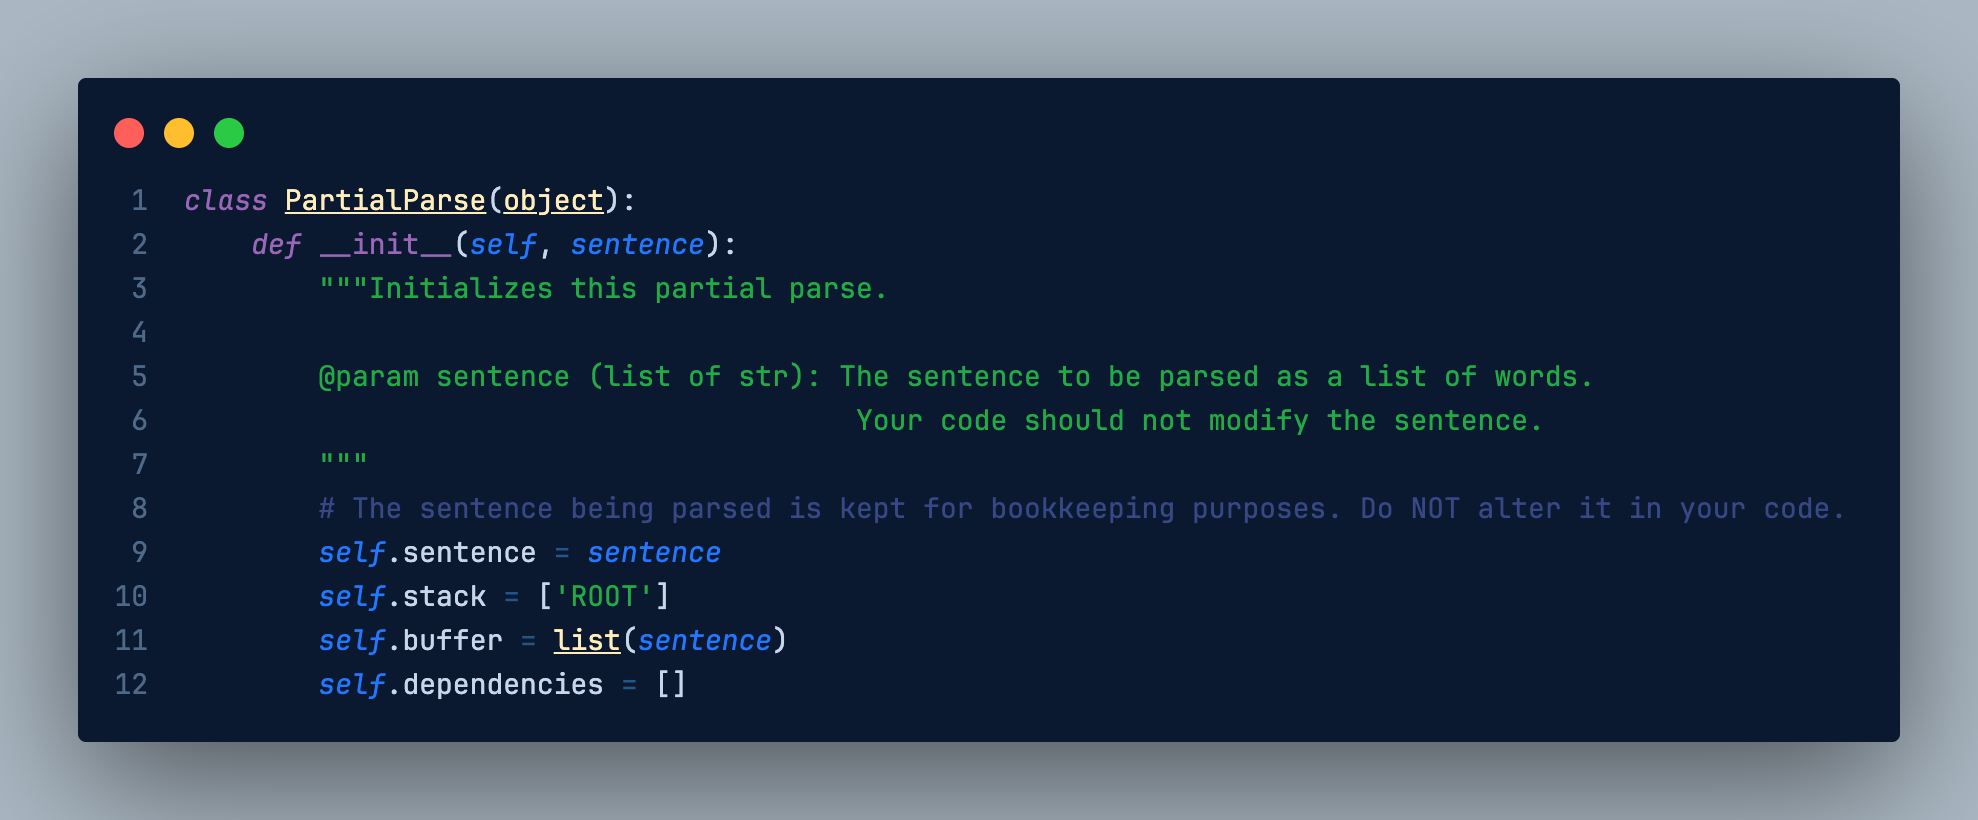
\includegraphics[width=0.82\linewidth,height=0.68\textheight,keepaspectratio]{../../assets/img/posts/cs224n-assignment-2/code2.png}
\caption{Parser implementation (first excerpt).}
\end{figure}

\begin{figure}[H]
\centering
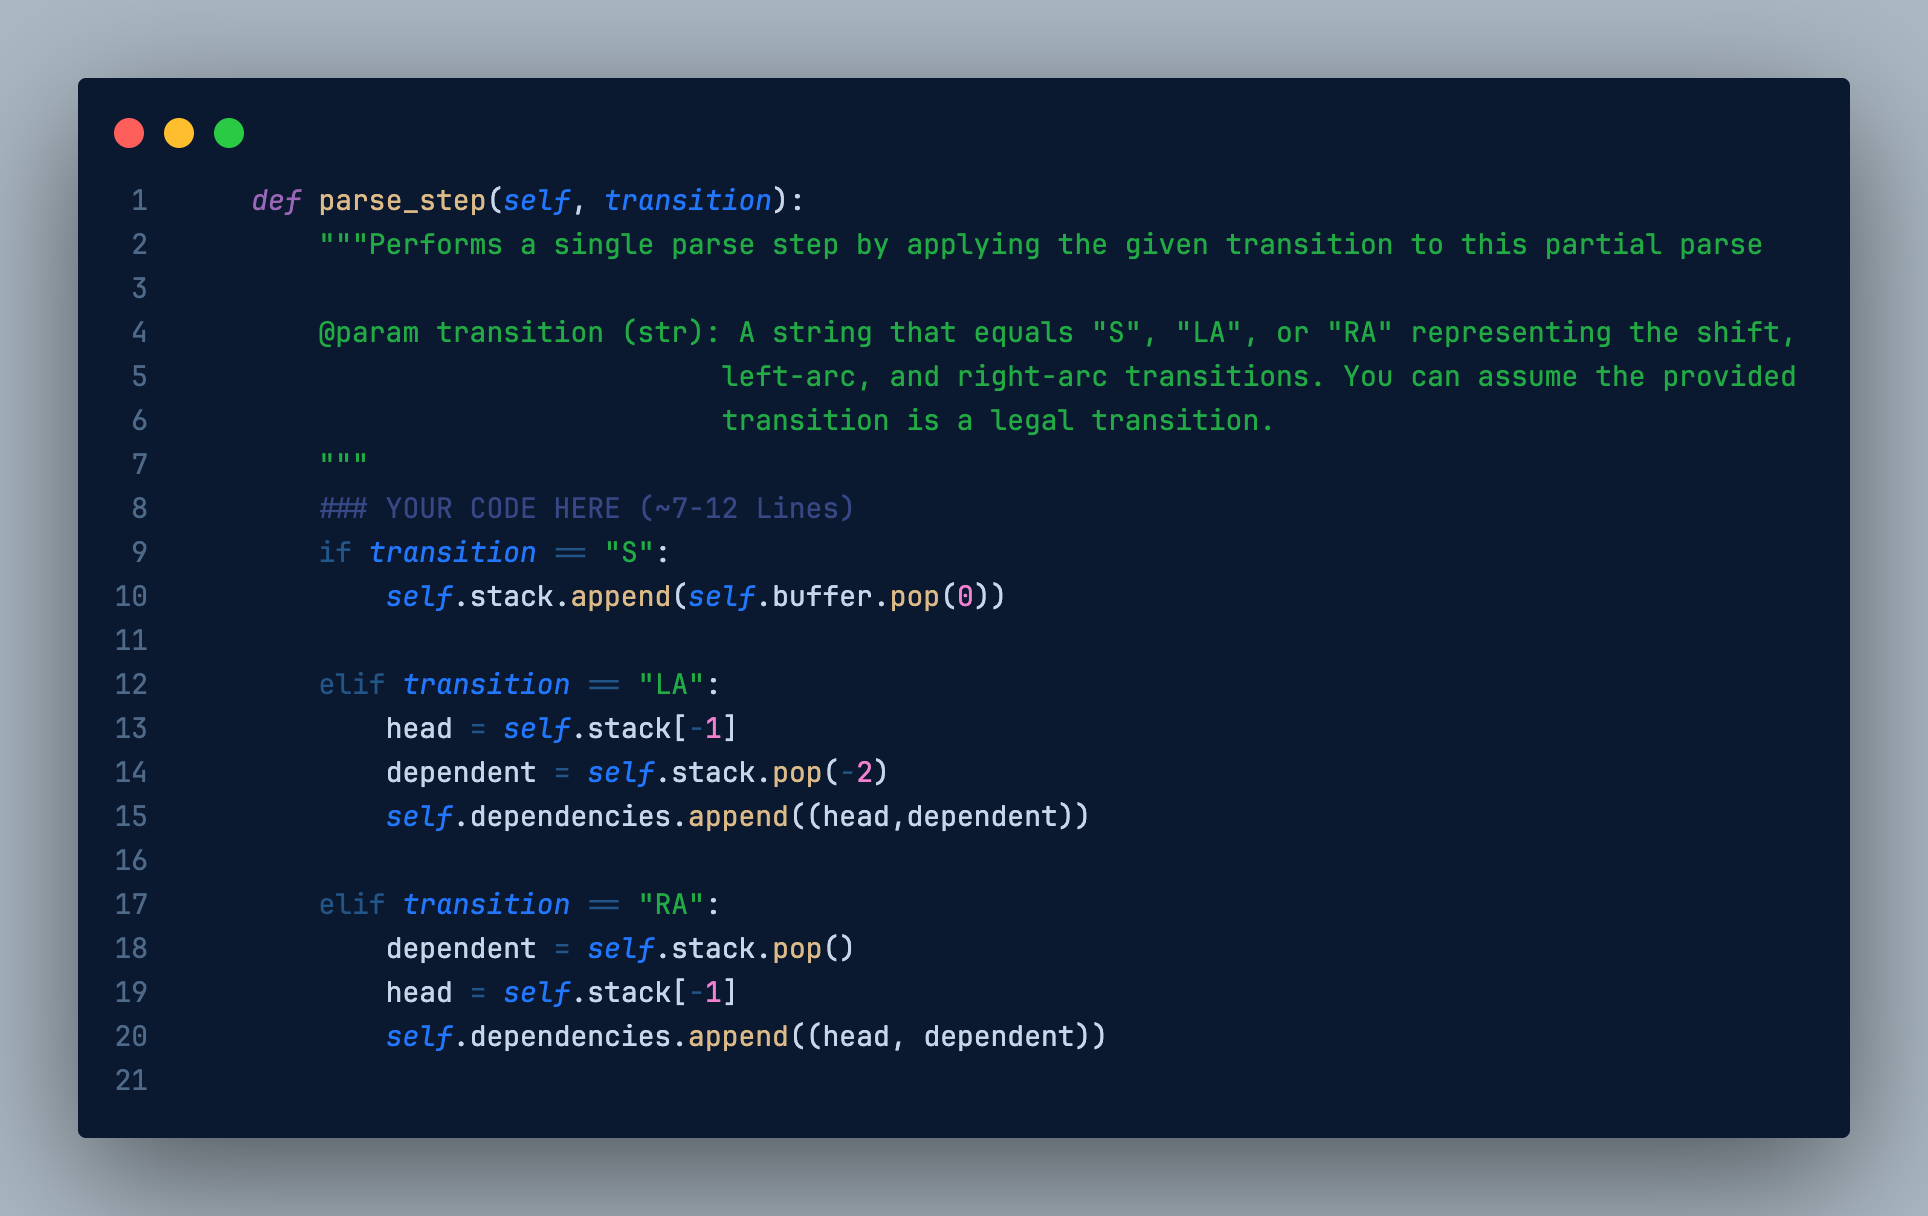
\includegraphics[width=0.75\linewidth,height=0.68\textheight,keepaspectratio]{../../assets/img/posts/cs224n-assignment-2/code.png}
\caption{PartialParse transition implementation.}
\end{figure}

\subsection{(d)}\label{d-1}

\texttt{minibatch\_parse} creates one \texttt{PartialParse} object for each input sentence and keeps their original order. During each iteration, it selects up to \texttt{batch\_size} unfinished parses, asks the model to predict one transition for each parse, and applies those transitions. A parse is removed from the unfinished list only when its buffer is empty and its stack contains only \texttt{ROOT}. Finally, dependencies are collected from the original list of partial parses, which preserves the input sentence order.

\begin{center}
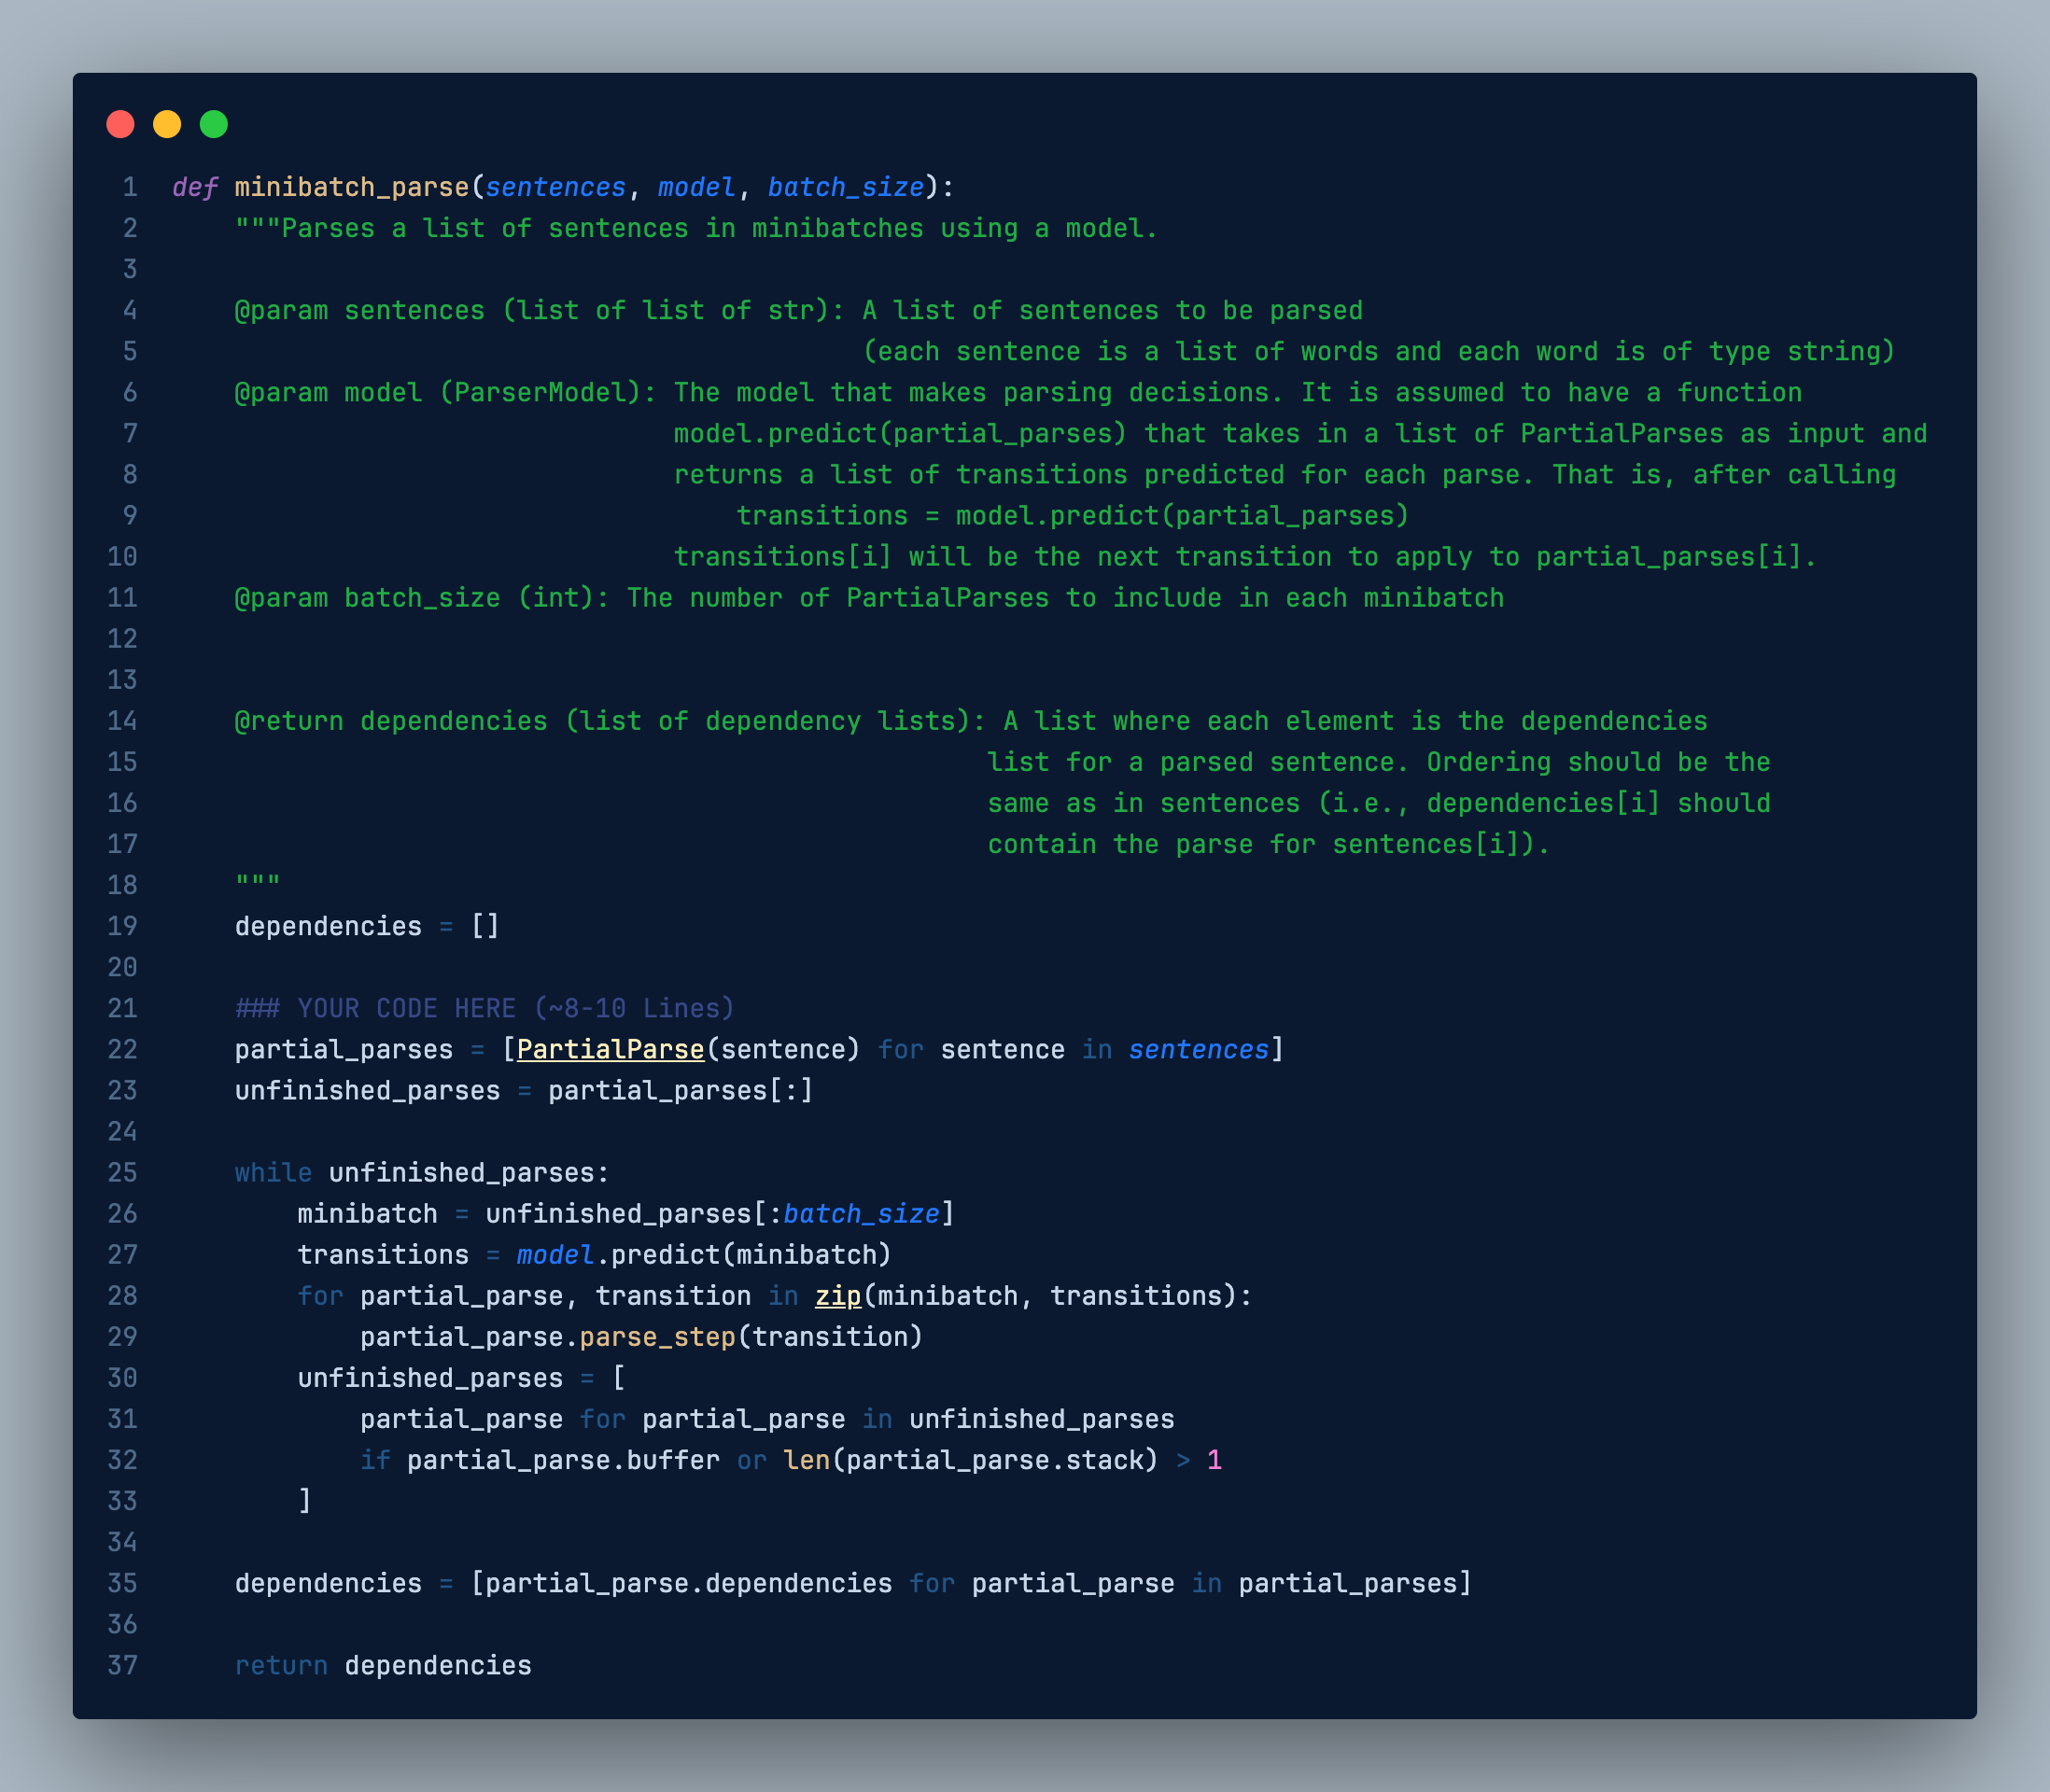
\includegraphics[width=0.80\linewidth,height=0.68\textheight,keepaspectratio]{../../assets/img/posts/cs224n-assignment-2/code3.png}
\end{center}

\subsection{(e)}\label{e-1}

\textbf{(i)}

Let

\[
\mathbf{z} = \mathbf{xW} + \mathbf{b}_1,
\qquad
\mathbf{h} = \operatorname{ReLU}(\mathbf{z}).
\]

For an individual hidden unit \(h_i\),

\[
h_i = \max(z_i, 0)
= \max\left(\sum_k x_k W_{ki} + b_{1,i}, 0\right).
\]

Therefore, for an input feature \(x_j\),

\[
\begin{cases}
W_{ji}, & z_i > 0,\\
0, & z_i < 0.
\end{cases}
\]

The derivative is undefined at \(z_i=0\), which the question allows us to ignore.

\textbf{(ii)}

Let the logits be \(\mathbf{l}\), and let

\[
\hat{y}_j = \frac{e^{l_j}}{\sum_k e^{l_k}}
\]

be the softmax probability for class \(j\). The cross-entropy loss is

\[
-\sum_j y_j \log \hat{y}_j.
\]

For a one-hot target vector whose correct class is \(c\), the derivative with respect to logit \(l_i\) is

\[
\hat{y}_i - y_i.
\]

Equivalently,

\[
\begin{cases}
\hat{y}_i - 1, & i=c,\\
\hat{y}_i, & i\neq c.
\end{cases}
\]

This gradient increases the logit of the correct transition and decreases the relative preference for incorrect transitions during training.

\textbf{(iii) UAS}

\begin{center}
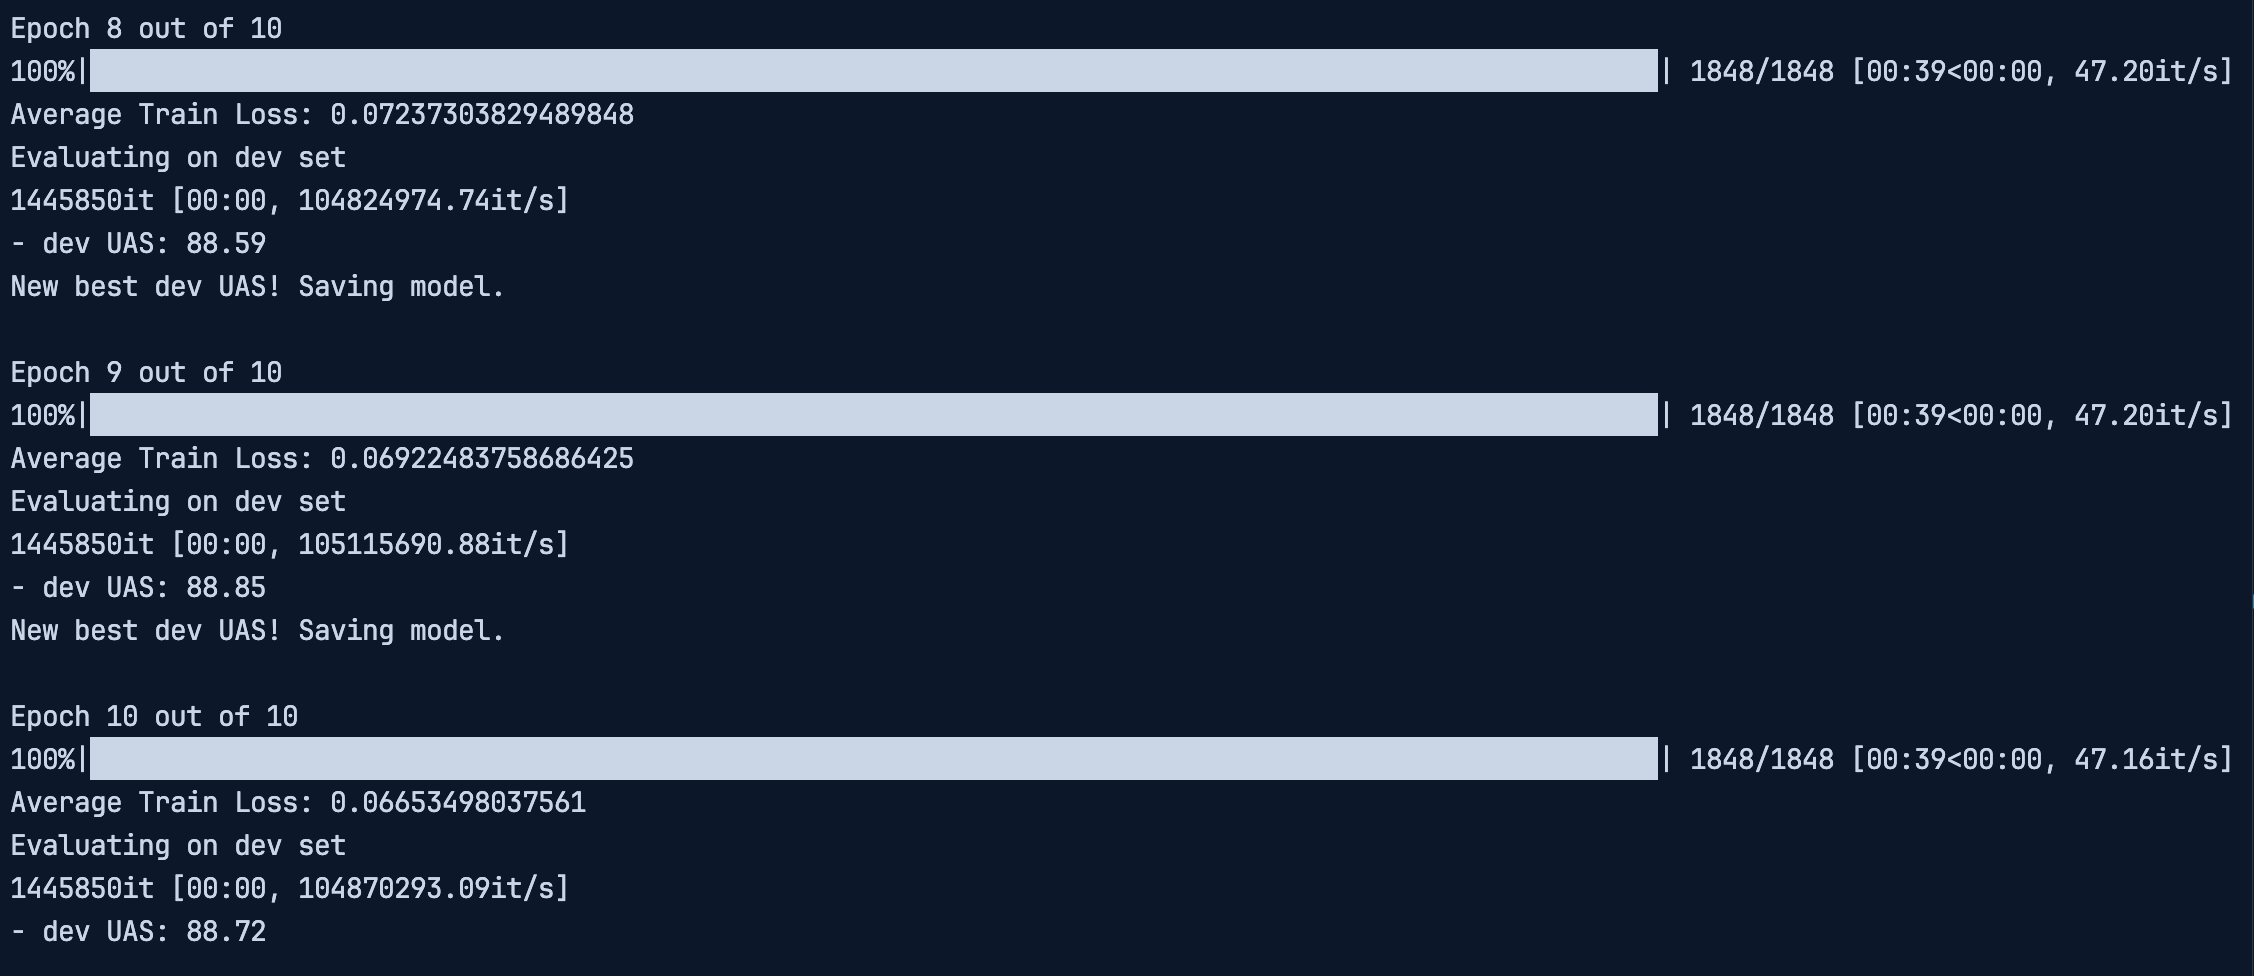
\includegraphics[width=0.94\linewidth,height=0.68\textheight,keepaspectratio]{../../assets/img/posts/cs224n-assignment-2/screenshot-2026-09-14-19-40-52.png}
\end{center}

\begin{center}
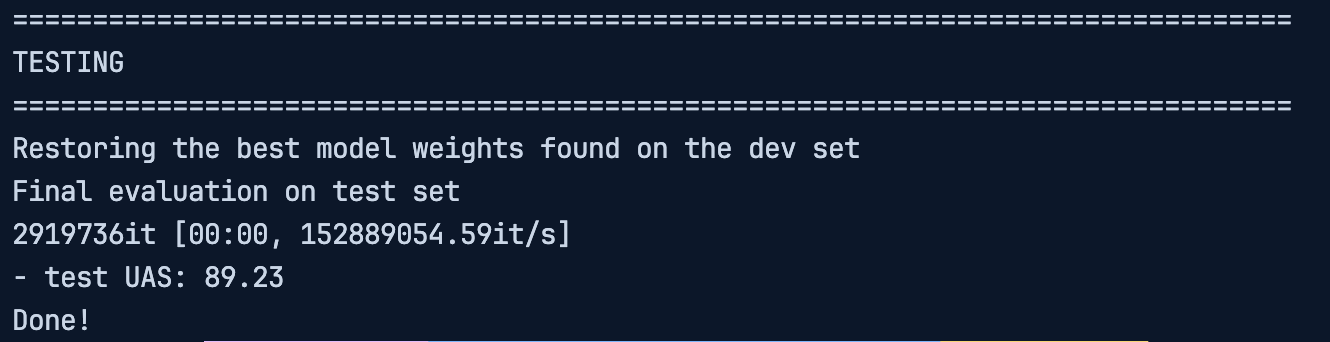
\includegraphics[width=0.94\linewidth,height=0.68\textheight,keepaspectratio]{../../assets/img/posts/cs224n-assignment-2/screenshot-2026-09-14-19-39-50.png}
\end{center}

The best development-set UAS achieved by the model was \textbf{88.85}. The final model, restored using the best development-set checkpoint, achieved a test-set UAS of \textbf{89.23}.

UAS measures the percentage of words whose predicted syntactic heads are correct, regardless of dependency-relation labels.

\subsection*{My code}

\begin{figure}[H]
\centering
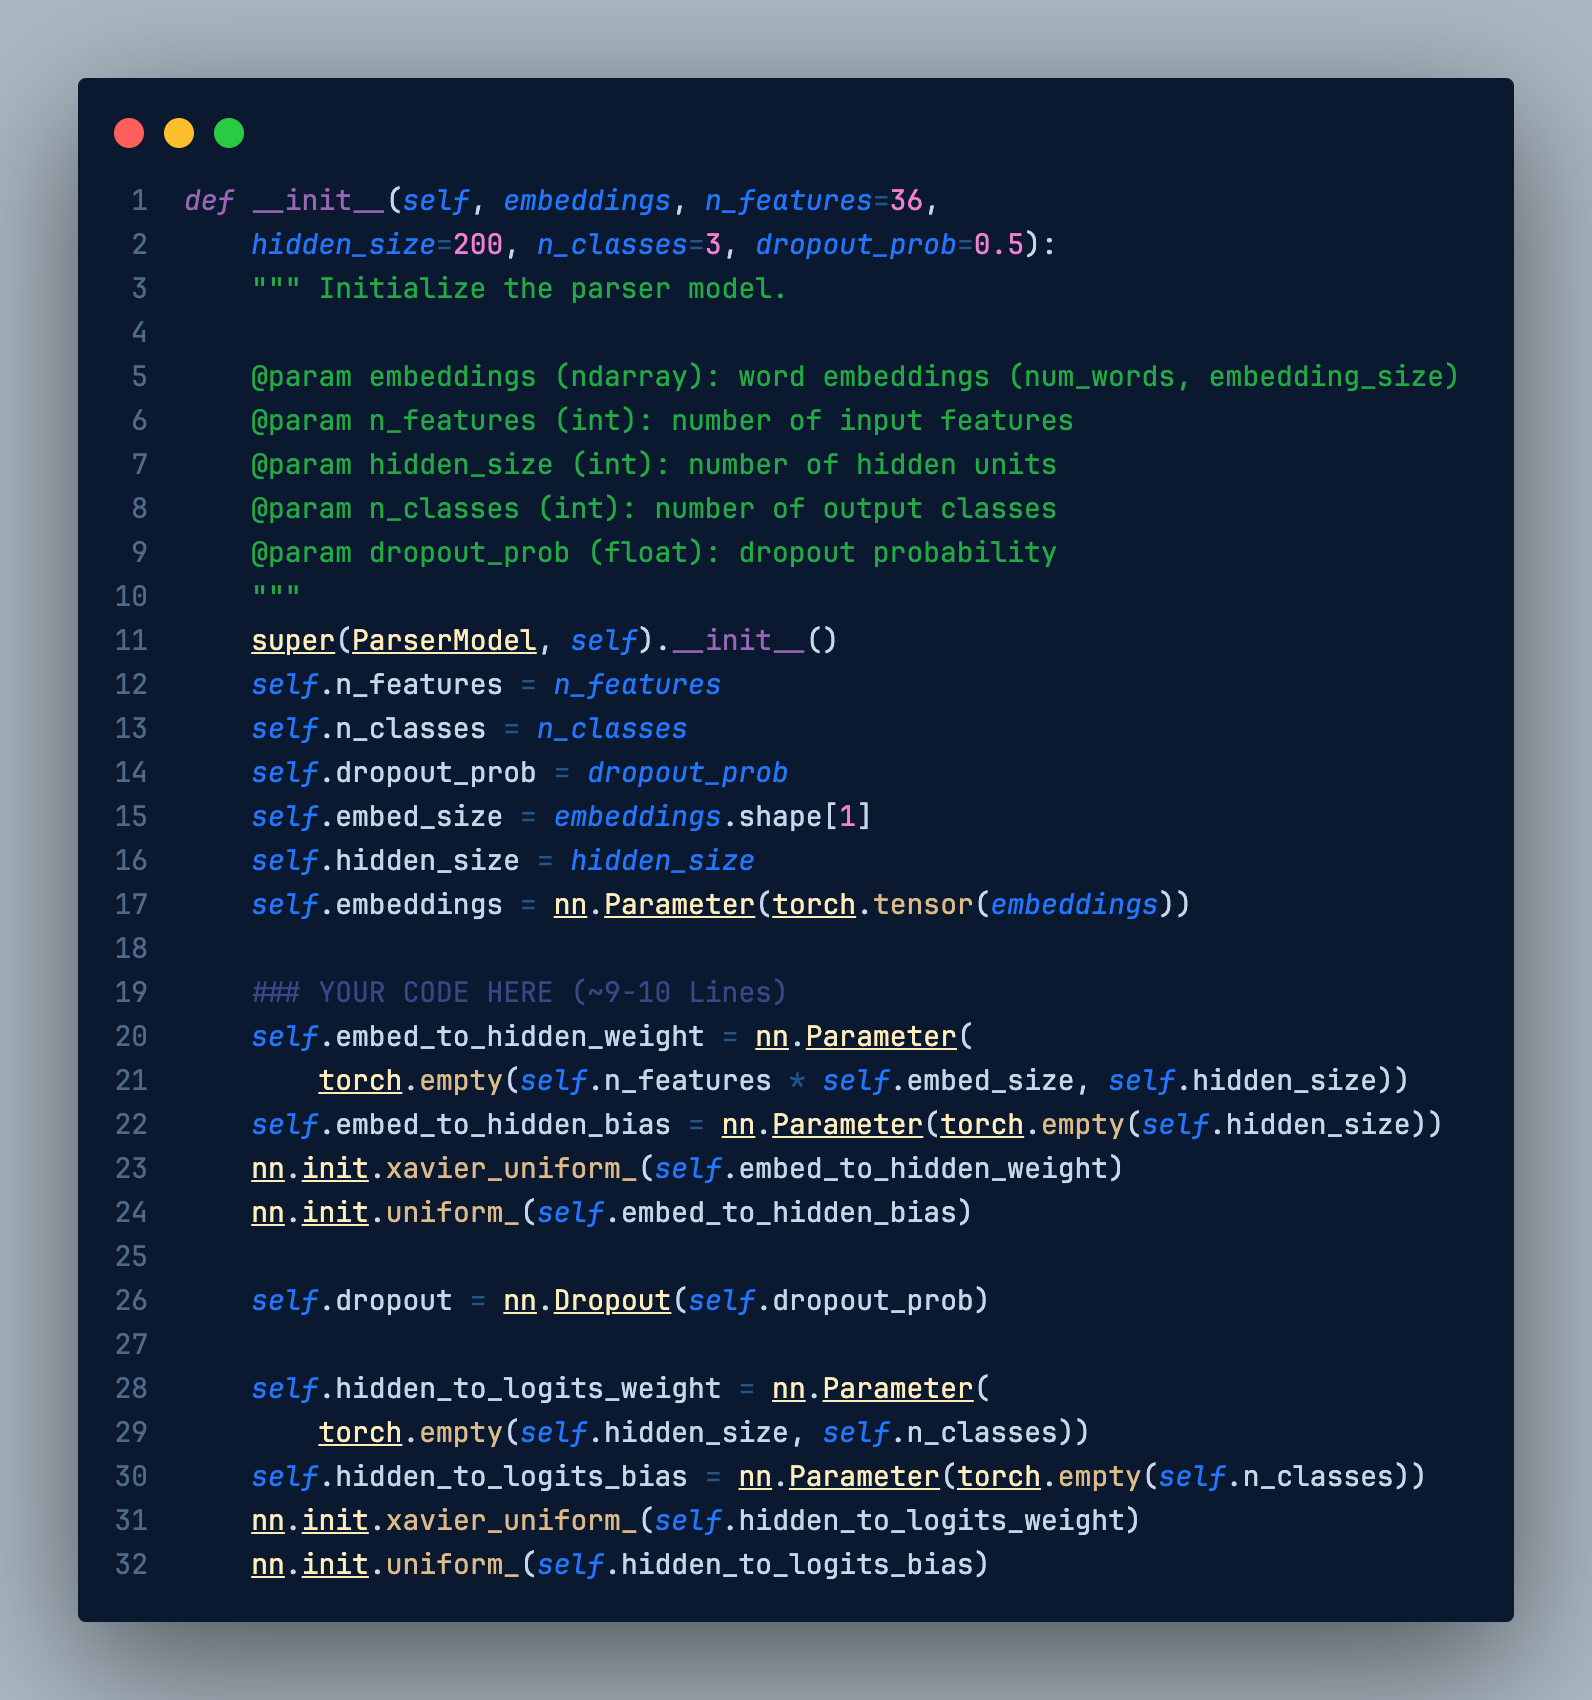
\includegraphics[width=0.88\linewidth,height=0.68\textheight,keepaspectratio]{../../assets/img/posts/cs224n-assignment-2/code4.png}
\caption{Parser model initialization.}
\end{figure}

\begin{center}
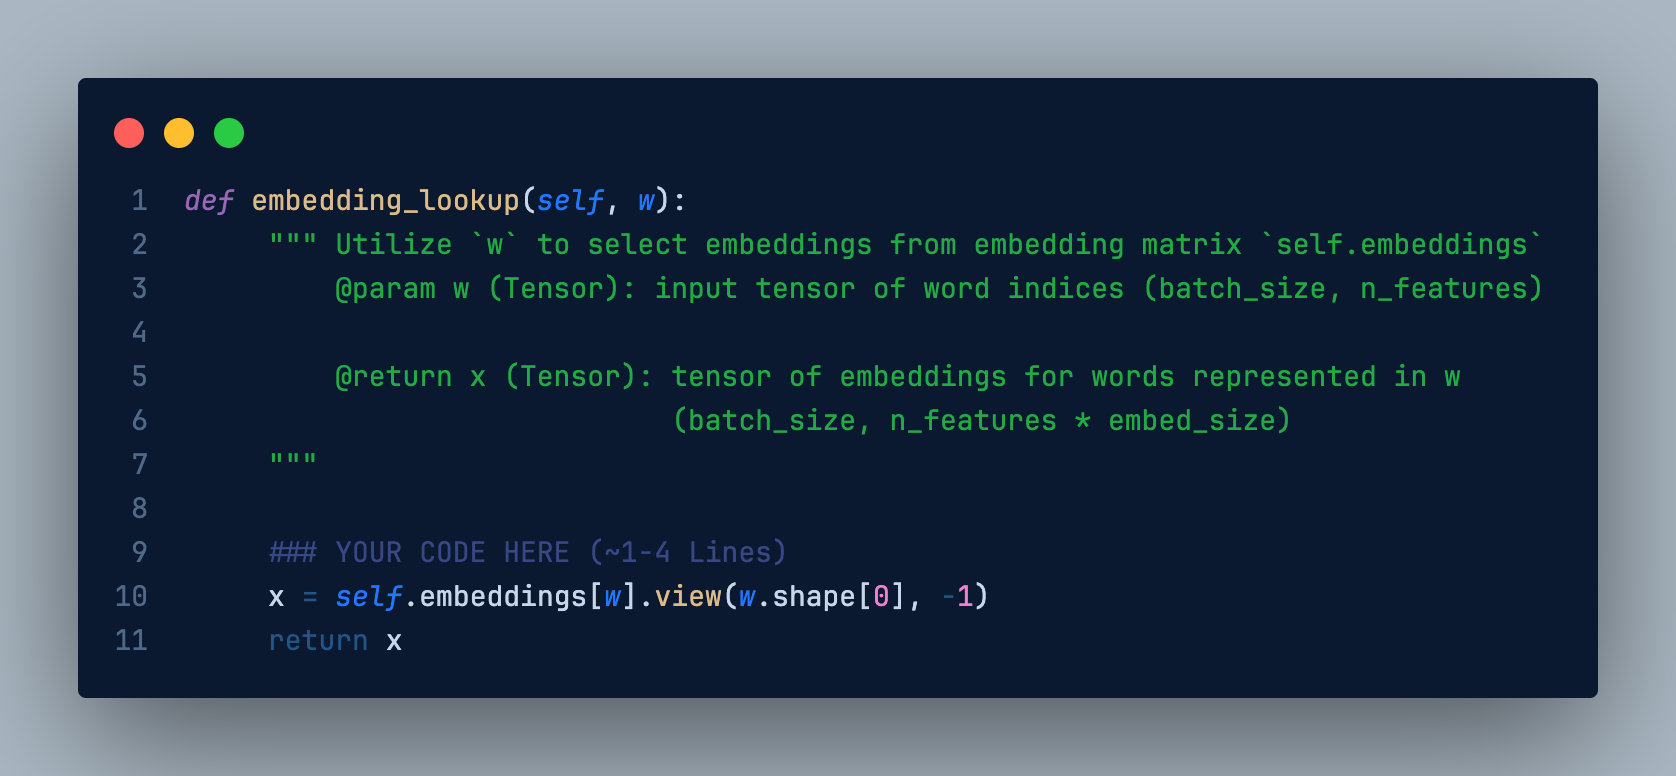
\includegraphics[width=0.85\linewidth,height=0.68\textheight,keepaspectratio]{../../assets/img/posts/cs224n-assignment-2/code5.png}
\end{center}

\begin{center}
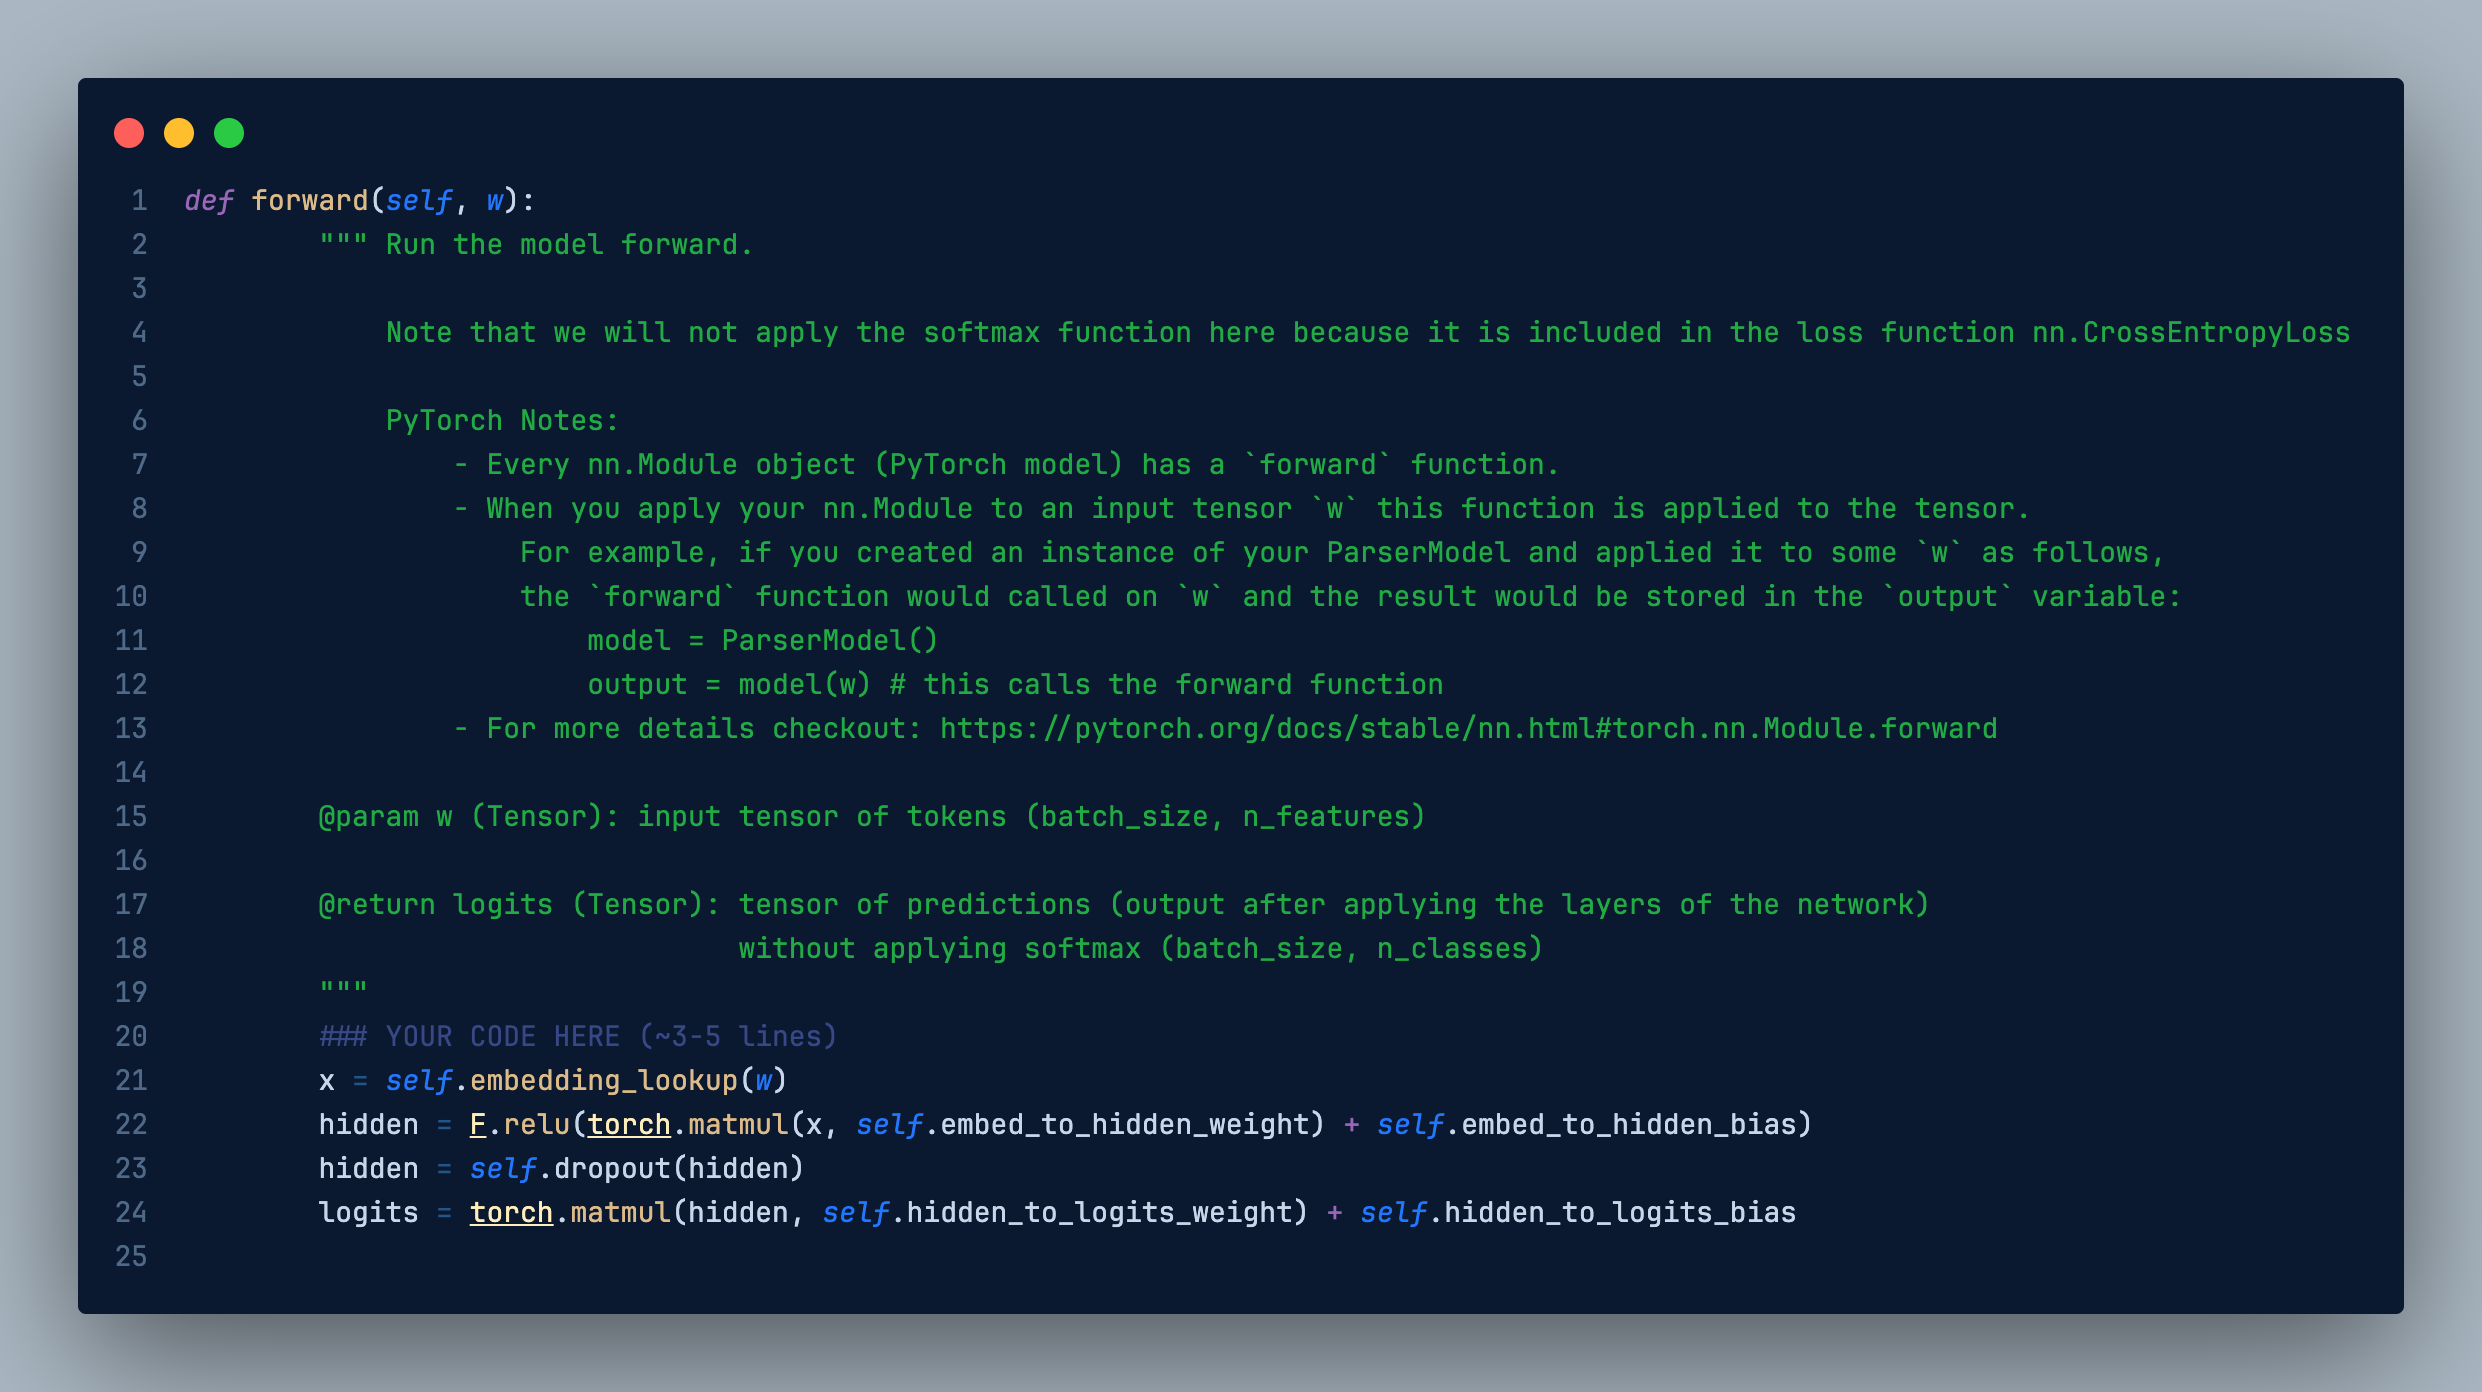
\includegraphics[width=0.94\linewidth,height=0.68\textheight,keepaspectratio]{../../assets/img/posts/cs224n-assignment-2/code6.png}
\end{center}

\subsection*{Test}

\begin{center}
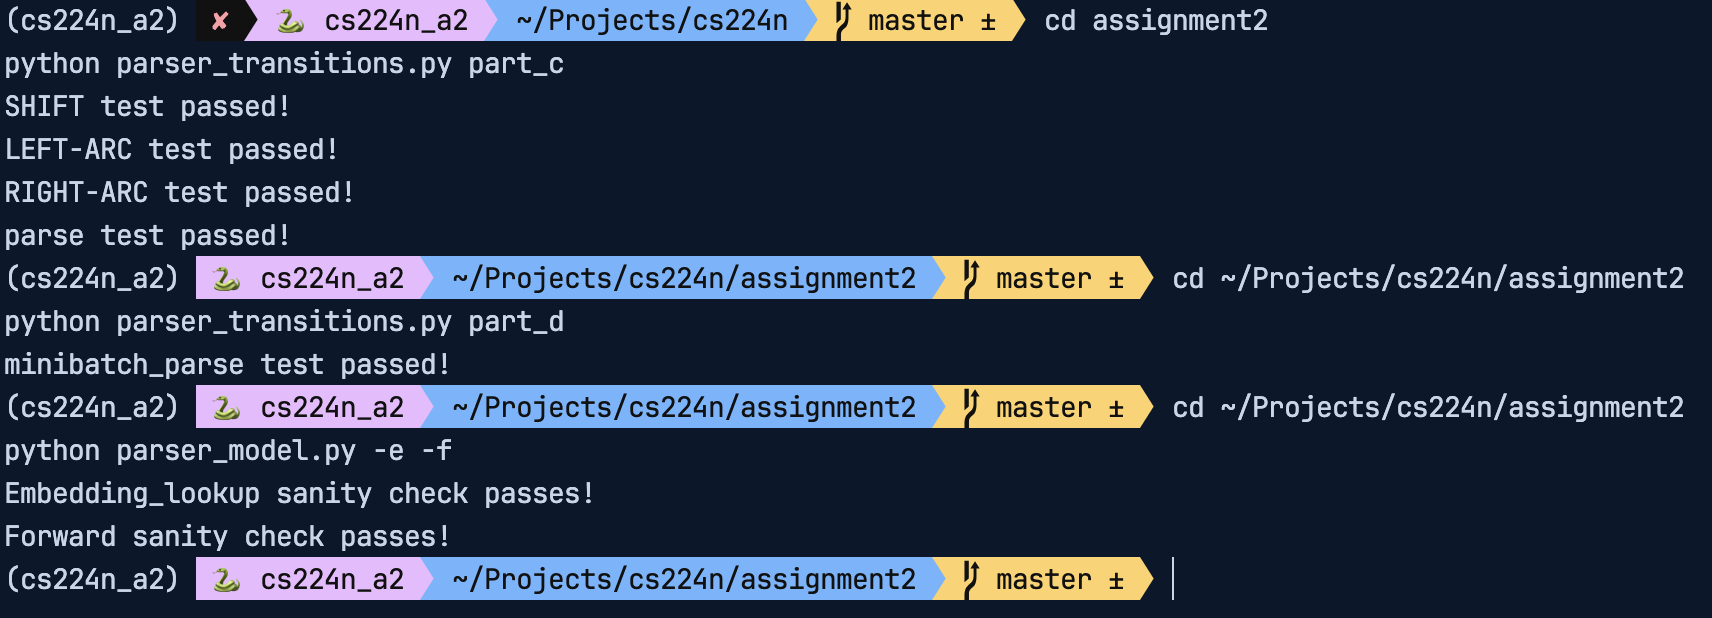
\includegraphics[width=0.94\linewidth,height=0.68\textheight,keepaspectratio]{../../assets/img/posts/cs224n-assignment-2/screenshot-2026-09-14-19-21-52.png}
\end{center}

\end{document}
